\documentclass{article}
\usepackage{amsmath}
\usepackage{amssymb}
\usepackage{graphicx}
\usepackage{float}

% Macros for common symbols
\newcommand{\Mp}{M_{\mathrm{P}}}
\newcommand{\rhom}{\rho_m}
\newcommand{\rhor}{\rho_r}
\newcommand{\rhoL}{\rho_\Lambda}

\title{Modified Einstein Equations for Stigma Q-Torsion Theory}
\author{Mathematica Analysis Results}
\date{\today}

\begin{document}

\maketitle

\section{Overview}

This document describes the Mathematica analysis performed on the Stigma Q-torsion theory, specifically focusing on the computation of modified Einstein equations and the effective gravitational constant.

\section{Analysis Components}

The Mathematica project consists of several key files:

\begin{itemize}
    \item \texttt{StigmaEquationsOfMotion.m} - Defines the FLRW spacetime and derives the equations of motion
    \item \texttt{ModifiedEinstein.m} - Computes the modified Einstein constant and effective gravitational coupling
    \item \texttt{DefManifold.m} - Sets up the manifold definitions using xAct
\end{itemize}

\section{Theory}
\subsection{Distances}
\subsubsection{Transverse Comoving Distance}
Transverse comoving distance is defined as:
\begin{equation}
		D_M(z) = \frac{c}{H_0 \sqrt{\Omega_k}} \sinh\left(\sqrt{\Omega_k} \int_0^z \frac{H_0}{H(z')} dz'\right)
\end{equation}
Comoving distance is the distance between two points that will remain constant with time if the points are moving with the Hubble flow. $D_M(z)$ is the transverse comoving distance, which is the comoving distance between two events at the same redshift or distance but separated on the sky by some angle. $D_M(z)$ specifically relates an observed angular separation on the sky to the corresponding comoving transverse separation at redshift $z$. It is related to the angular diameter distance $D_A(z)$ and luminosity distance $D_L(z)$ by the following equations:
\begin{equation}
		D_A(z) = \frac{D_M(z)}{1+z} = \frac{l}{\theta}.
\end{equation}
The angular diameter distance is defined as the ratio of an object's physical transverse size $l$ to its angular size $\theta$ (in radians). It is therefore the distance that converts an observed angular size into the corresponding physical size of an object at redshift $z$. 
The luminosity distance is defined as the distance that relates the observed flux $F$ from a source to its intrinsic luminosity $L$ via the inverse square law:
\begin{equation}
		D_L(z) = (1+z) D_M(z) = \sqrt{\frac{L}{4 \pi F}},
\end{equation}
it is therefore the distance that an object would appear to have in a static Euclidean universe producing the same observed flux.
Combining them gives the distance duality relation:
\begin{equation}
		D_L(z) = (1+z)^2 D_A(z)
\end{equation}

\subsubsection{Sound Horizon at drag epoch -- BAO Ruler}
BAO depends on the sound horizon at drag epoch. It is the distance that sound can travel between the Big Bang and the drag epoch, which is when baryons are released from photons. It is given by the following integral:
\begin{equation}
		r_d = \int_{z_d}^\infty \frac{c_s(z)}{H(z)} dz,
\end{equation}
where $c_s(z)$ is the sound speed of the photon-baryon fluid. When $z > z_d$, the photons couple to baryons via compton scattering. It had coulomb interactions with the baryons. $z_d$ is about 1060, in comparison to the redshift of recombination $z_*$ which is about 1090. It happened later becasue there are so few baryons in comparison to photons. Even after recombination, there are still enough free electrons left that photons continue to exert a small pressure on baryons through Thomson scattering. In recombination: electron and proton combine to form neutral hydrogen, but there are still free electrons left that can scatter photons. In drag epoch: the photon pressure on baryons becomes negligible, and baryons are effectively released from the photons -- BAO ruler freezes in.

\subsubsection{Hubble Distance}
The Hubble distance is defined as:
\begin{equation}
		D_H(z) = \frac{c}{H(z)},
\end{equation}
it is the distance that light can travel in one Hubble time at redshift $z$. It is a characteristic scale that sets the expansion rate of the universe at that redshift. It is often used as a reference scale for cosmological measurements, such as in BAO analyses where distances are often expressed in units of the Hubble distance.

\subsubsection{Angle-averaged Distance}
The angle-averaged distance is defined as:
\begin{equation}
		D_V(z) = \left[ z D_M(z)^2 D_H(z) \right]^{1/3},
\end{equation}
it quantifies the average of the distances measured along, and perpendicular to the line of sight of the observer. It is used in BAO analyses to combine measurements of the transverse and radial BAO scales into a single distance measure that can be compared to theoretical predictions.

\subsection{BAO}
Baryon Acoustic Oscillations (BAO) are periodic fluctuations in the density of visible baryonic matter (normal matter) of the universe. They are caused by acoustic waves that propagated through the early universe when photons and baryons were tightly coupled. The sound waves created regions of higher and lower density in the matter distribution, which left an imprint on the large-scale structure of the universe. The characteristic scale of these oscillations is determined by the sound horizon at the drag epoch, which is the distance that sound could travel in the early universe before baryons were released from photons. This scale serves as a "standard ruler" for measuring cosmological distances, allowing us to probe the expansion history of the universe and constrain cosmological parameters.

BAO measurement constrains $D_M(z)/r_d$ and $D_H(z)/r_d$. The transverse BAO scale is related to the angular diameter distance $D_A(z)$, while the radial BAO scale is related to the Hubble distance $D_H(z)$. By measuring the BAO scale in both directions, we can obtain constraints on the expansion history of the universe and the underlying cosmological model.

To understand this better: This sound wave is not between baryons but rather the photon-baryonic sound wave. Baryons have gravity and therefore exert an attractive force, whereas photons pushes things out through radiation pressure: photo interacts with electrons through Thompson scattering, the electrons then pushes baryons out through coulomb interaction. The sound wave is the result of the competition between these two forces. When the universe was hot and dense, photons were tightly coupled to baryons, and the sound wave propagated through this photon-baryon fluid. As the universe expanded and cooled, photons decoupled from baryons at the drag epoch.



\section{Key Results}

\subsection{Series-Expanded Equations of Motion}

Applying \texttt{MakeSeries} to the final equations (\texttt{EqnFinal} and \texttt{EqVarpiFinal}) expresses them in conformal time $\tau$ with the matter content written in terms of the density parameters $\{\Omega_{r,0}, \Omega_{m,0}, \Omega_{\Lambda,0}\}$. Below, $a \equiv a(\tau)$, $\varpi \equiv \varpi(\tau)$, and primes denote $d/d\tau$. The Mathematica symbols map to the notation used here as
\begin{equation}
\texttt{stigma} = \varsigma, \qquad
\texttt{mups2} = -\upsilon_2, \qquad
\texttt{alps} = \alpha \to 1,
\end{equation}
i.e.\ the scale-factor normalisation \texttt{alps} is set to unity and suppressed throughout.

\subsubsection{Constraint Equation}

The constraint equation \texttt{ConstraintEqn} reads $\mathcal{C} = 0$ with

\begin{equation}
\begin{aligned}
\mathcal{C} = {}& -\frac{3 H_0^2 \Mp^2 \left(\Omega_{r,0} + \Omega_{m,0}\, a + \Omega_{\Lambda,0}\, a^4\right)}{a} \\
&- \frac{3 \Mp^2 \upsilon_2 \left(4 \varsigma - \varpi^2\right) a'^2}{4 \varsigma\, a}
+ \frac{3 \Mp^2 \upsilon_2\, \varpi\, a'\, \varpi'}{2 \varsigma}
+ \frac{3 \Mp^2 \upsilon_2\, a\, \varpi'^2}{4 \varsigma} \\
&+ \frac{3 \Mp^2 \upsilon_2\, \varsigma\, a}{\varsigma - \varpi^2}
   \left(\frac{\left(\varpi^2 - 1\right) a'}{a} + \varpi\, \varpi'\right)^2 .
\end{aligned}
\end{equation}

\subsubsection{$\varpi$ Field Equation}

The $\varpi$ equation of motion \texttt{VarPiEqn} reads $\mathcal{V} = 0$ with

\begin{equation}
\begin{aligned}
\mathcal{V} = {}& \frac{3 \Mp^2 \upsilon_2 \left(1 - 4 \varsigma^2\right) \varpi^5\, a''}{2 \varsigma \left(\varsigma - \varpi^2\right)^2} \\
&+ \frac{3 \Mp^2 \upsilon_2\, \varsigma\, \varpi \left(4 (\varsigma - 1)\, a'^2 + 4 \varsigma\, a^2 \varpi'^2 + (1 - 4 \varsigma)\, a\, a''\right)}{2 a \left(\varsigma - \varpi^2\right)^2} \\
&+ \frac{3 \Mp^2 \upsilon_2\, \varpi^3 \left(-2 \varsigma (\varsigma - 1)\, a'^2 + \left(2 \varsigma (1 + \varsigma) - 1\right) a\, a''\right)}{a \left(\varsigma - \varpi^2\right)^2} \\
&+ \frac{3 \Mp^2 \upsilon_2\, \varsigma \left(2 a' \varpi' + a\, \varpi''\right)}{2 \left(\varsigma - \varpi^2\right)^2}
+ \frac{3 \Mp^2 \upsilon_2 \left(2 \varsigma^2 - 1\right) \varpi^2 \left(2 a' \varpi' + a\, \varpi''\right)}{\left(\varsigma - \varpi^2\right)^2} \\
&- \frac{3 \Mp^2 \upsilon_2 \left(4 \varsigma^2 - 1\right) \varpi^4 \left(2 a' \varpi' + a\, \varpi''\right)}{2 \varsigma \left(\varsigma - \varpi^2\right)^2} .
\end{aligned}
\end{equation}

Collecting the common prefactor $3 \Mp^2 \upsilon_2 / \left[2 \varsigma (\varsigma - \varpi^2)^2\right]$ and grouping the $\left(2 a' \varpi' + a \varpi''\right)$ terms:

\begin{equation}
\begin{aligned}
\mathcal{V} = \frac{3 \Mp^2 \upsilon_2}{2 \varsigma \left(\varsigma - \varpi^2\right)^2} \Big[
& \left(1 - 4 \varsigma^2\right) \varpi^5 a'' \\
&+ \frac{\varsigma^2 \varpi}{a}\left(4 (\varsigma - 1) a'^2 + 4 \varsigma a^2 \varpi'^2 + (1 - 4 \varsigma) a\, a''\right) \\
&+ \frac{2 \varsigma \varpi^3}{a}\left(-2 \varsigma (\varsigma - 1) a'^2 + \left(2 \varsigma (1 + \varsigma) - 1\right) a\, a''\right) \\
&+ \left(\varsigma^2 + 2 \varsigma \left(2 \varsigma^2 - 1\right) \varpi^2 - \left(4 \varsigma^2 - 1\right) \varpi^4\right) \\
&\qquad \times \left(2 a' \varpi' + a\, \varpi''\right)
\Big] .
\end{aligned}
\end{equation}

\subsubsection{Power Series Substitution}

To solve $\mathcal{C} = 0$ and $\mathcal{V} = 0$ order by order at early times, we substitute the truncated power series
\begin{align}
a(\tau) &\to a_1 \tau + a_2 \tau^2 + a_3 \tau^3 + a_4 \tau^4 + a_5 \tau^5, \\
\varpi(\tau) &\to 1 + \varpi_1 \tau + \varpi_2 \tau^2 + \varpi_3 \tau^3 + \varpi_4 \tau^4,
\end{align}
where $a_i \equiv \texttt{ScaleFactor}i$ (Mathematica \texttt{ScaleFactor1}, \texttt{ScaleFactor2}, \dots) and $\varpi_i \equiv \texttt{VarPi}i$ (\texttt{VarPi1}, \texttt{VarPi2}, \dots). Note that $a(\tau)$ has no constant term, so the expansion starts at $\mathcal{O}(\tau)$ and $a(0) = 0$, while $\varpi(\tau)$ is normalised to $\varpi(0) = 1$. The resulting derivatives are
\begin{align}
a'(\tau) &= a_1 + 2 a_2 \tau + 3 a_3 \tau^2 + 4 a_4 \tau^3 + 5 a_5 \tau^4, \\
a''(\tau) &= 2 a_2 + 6 a_3 \tau + 12 a_4 \tau^2 + 20 a_5 \tau^3, \\
\varpi'(\tau) &= \varpi_1 + 2 \varpi_2 \tau + 3 \varpi_3 \tau^2 + 4 \varpi_4 \tau^3, \\
\varpi''(\tau) &= 2 \varpi_2 + 6 \varpi_3 \tau + 12 \varpi_4 \tau^2 .
\end{align}
Inserting these into $\mathcal{C}$ and $\mathcal{V}$, expanding in $\tau$, and demanding that each coefficient vanish independently yields an algebraic system for the nine coefficients $\{a_1, \ldots, a_5\}$ and $\{\varpi_1, \ldots, \varpi_4\}$ in terms of the theory parameters $\{\varsigma, \upsilon_2\}$ and the cosmological densities $\{\Omega_{r,0}, \Omega_{m,0}, \Omega_{\Lambda,0}\}$.

% \subsection{Equations of Motion}

% \subsubsection{Lapse Function Equation}

% \begin{equation}
% \begin{aligned}
% 0 &= \frac{a}{4 \varsigma} \Big[ \frac{12 \upsilon _2 \varsigma^2 \Mp^2 \left(\left(\varpi^2-1\right) a' + a \varpi \varpi'\right)^2}{\varsigma-\varpi^2} \\
% &\quad + 6 \upsilon _2 a \Mp^2 \varpi a' \varpi' + 3 \upsilon _2 \Mp^2 a'^2 \left(\varpi^2-4 \varsigma\right) \\
% &\quad - 4 \varsigma a^2 \left(\rhom+\rhor+\rhoL\right) + 3 \upsilon _2 a^2 \Mp^2 \varpi'^2 \Big]
% \end{aligned}
% \end{equation}

% \subsubsection{Scale Factor Equation}

% \begin{equation}
% \begin{aligned}
% 0 &= \frac{3}{4 \varsigma} \Big[ \frac{12 \upsilon _2 \varsigma^2 \Mp^2 \left(\left(\varpi^2-1\right) a' + a \varpi \varpi'\right)^2}{\varsigma-\varpi^2} \\
% &\quad + \upsilon _2 \Mp^2 a'^2 \left(\varpi^2-4 \varsigma\right) + 2 \upsilon _2 a \Mp^2 \left(a'' \left(\varpi^2-4 \varsigma\right)+2 \varpi a' \varpi'\right) \\
% &\quad - \upsilon _2 a^2 \Mp^2 \left(\varpi'^2-2 \varpi \varpi''\right) + \frac{4}{3} \varsigma a^2 \rhor - 4 \varsigma a^2 \rhoL \Big]
% \end{aligned}
% \end{equation}

% \subsubsection{Varpi Field Equation}

% \begin{equation}
% \begin{aligned}
% 0 &= \frac{3 \upsilon _2 a \Mp^2}{2 \varsigma \left(\varsigma-\varpi^2\right)^2} \Big[ a \left(3 a' \varpi' + a \varpi''\right) \left(\varsigma^2 + 2 \varsigma \left(2 \varsigma^2-1\right) \varpi^2 - \left(4 \varsigma^2-1\right) \varpi^4\right) \\
% &\quad + \varsigma^2 \varpi \left((1-4 \varsigma) a a'' - 3 a'^2 + 4 \varsigma a^2 \varpi'^2\right) \\
% &\quad + 2 \varsigma \varpi^3 \left((2 \varsigma (\varsigma+1)-1) a a'' + (4 \varsigma-1) a'^2\right) \\
% &\quad - \left(4 \varsigma^2-1\right) \varpi^5 \left(a a'' + a'^2\right) \Big]
% \end{aligned}
% \end{equation}

\subsection{Effective Gravitational Constant Ratio}

The effective gravitational constant ratio $G_{\text{eff}}/G_{\text{GR}}$ for constant $\varpi$ is:

\begin{equation}
g_i = \frac{4 \varsigma \left(\varsigma-\varpi^2\right)}{\upsilon_2 \varpi^2 \left(4 \varsigma^2 \varpi^2-8 \varsigma^2+5 \varsigma-\varpi^2\right)}
\end{equation}

\subsection{Complex Solutions as Function of Equation of State}

When solving the full system with $w_i$ dependence, the gravitational constant ratio has three solutions:

\begin{equation}
g_i \in \left\{\text{ComplexInfinity}, g_i^-, g_i^+\right\}
\end{equation}

where:

\begin{equation}
\begin{aligned}
g_i^{\pm} &= \frac{4}{\varsigma \upsilon_2 (6 (\varsigma-1) w_i+2 \varsigma+1) (4 \varsigma (3 w_i+1)-3 w_i-7)} \\
&\quad \times \Big[ \varsigma^3 \left(-(3 w_i+1)^2\right) + \varsigma (3-9 w_i) + (3 \varsigma w_i+\varsigma)^2 \\
&\quad\quad \pm (3 w_i+1) \sqrt{(\varsigma-1)^2 \varsigma^2 \left((3 \varsigma w_i+\varsigma)^2-6 w_i+2\right)} \Big]
\end{aligned}
\end{equation}

where:
\begin{itemize}
    \item $\varsigma$ is the stigma parameter
    \item $w_i$ is the equation of state parameter
    \item $\upsilon_2$ is the coupling parameter
\end{itemize}

\subsection{Density Plots of Solutions}

The two non-infinite solution branches are visualized as density plots showing the behavior of $g_i^{\pm}$ in the $w_i$-$\varsigma$ parameter space.

\begin{figure}[H]
\centering
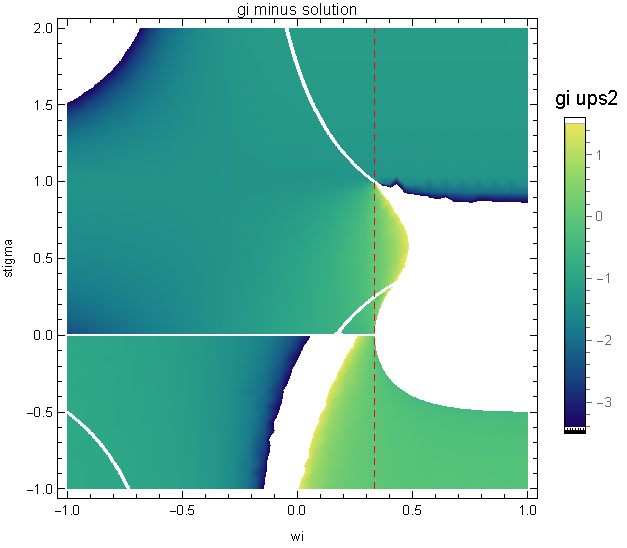
\includegraphics[width=0.8\textwidth]{gisolution_minus.pdf}
\caption{Density plot of $g_i^-$ solution as a function of equation of state parameter $w_i$ and stigma parameter $\varsigma$. The red dashed line indicates $w_i = 1/3$ (matter-radiation equality).}
\label{fig:gisolution_minus}
\end{figure}

\begin{figure}[H]
\centering
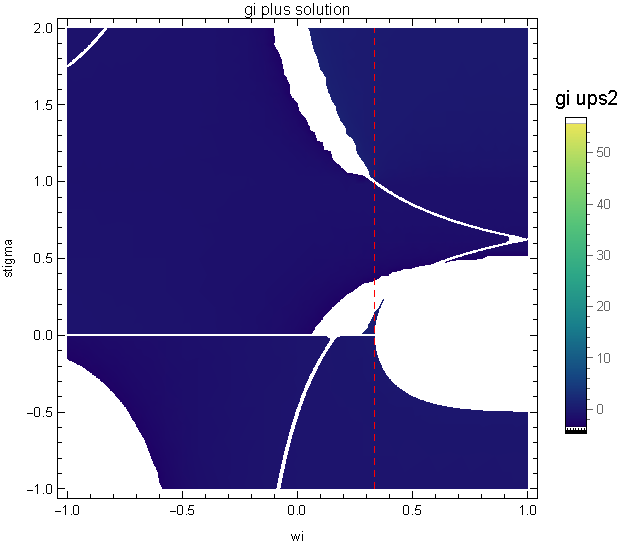
\includegraphics[width=0.8\textwidth]{gisolution_plus.pdf}
\caption{Density plot of $g_i^+$ solution as a function of equation of state parameter $w_i$ and stigma parameter $\varsigma$. The red dashed line indicates $w_i = 1/3$ (matter-radiation equality).}
\label{fig:gisolution_plus}
\end{figure}

\section{Todo Items}

\begin{enumerate}
    \item \textbf{Modified Friedmann equation with $G_{\text{newton}}$ baked in}
    \begin{itemize}
        \item Rewrite Friedmann equation incorporating the effective gravitational constant directly
        \item Make the modified gravity effects explicit in the cosmological dynamics
    \end{itemize}
    
    \item \textbf{Numerically extract $\varpi$ from GR Friedmann equation}
    \begin{itemize}
        \item Take standard GR Friedmann equation but replace $G_{\text{newton}}$ with our derived formula
        \item Compare numerical solutions with our fully solved analytical equations
        \item Validate consistency between approaches
    \end{itemize}
    
    \item \textbf{Interpolate between epochs and test numerically determined $w_i$}
    \begin{itemize}
        \item Study transitions between different cosmological epochs
        \item Test how the equation of state parameter $w_i$ varies
        \item Validate numerical interpolation methods
    \end{itemize}
    
    \item \textbf{PowerExpand implementation}
    \begin{itemize}
        \item Use PowerExpand appropriately in calculations to handle square roots
        \item Ensure proper treatment of complex expressions and absolute values
    \end{itemize}
    
    \item \textbf{Claude LaTeX conversion tool}
    \begin{itemize}
        \item Build Claude tool to convert .m file expressions to LaTeX verbatim
        \item Use InputForm to feed expressions to Claude
        \item Don't let Claude do math, just verbatim conversion
    \end{itemize}
    
    \item \textbf{Variable dictionary}
    \begin{itemize}
        \item Create mapping between Mathematica workflow variables and LaTeX notation
        \item Build systematic translation dictionary for consistent documentation
    \end{itemize}
\end{enumerate}

\subsection{Modified Friedmann Equations}

The analysis derives modified Friedmann equations for the Stigma Q-torsion theory by:
\begin{enumerate}
    \item Setting up FLRW metric with scale factor $a(t)$ and lapse function $N(t)$
    \item Applying steady-state assumptions ($\dot{\varpi} = 0$)
    \item Computing the Lagrangian with torsion modifications
    \item Deriving field equations through variational principle
\end{enumerate}

\section{Computational Method}

The calculation uses the xAct package for tensor computations and follows these steps:
\begin{enumerate}
    \item Load manifold definitions and set up FLRW spacetime
    \item Define scalar fields and their kinetic terms
    \item Construct the modified Lagrangian including torsion effects
    \item Apply Euler-Lagrange equations to derive field equations
    \item Solve for the effective gravitational constant under steady-state conditions
\end{enumerate}

\section{Early Time Power Series Solutions}

\subsection{Power Series Ansatz}

The early time power series expansion for the scale factor and $\varpi$ field in conformal time $\tau$ takes the form:

\begin{align}
a(\tau) &= a_1 \tau + a_2 \tau^2 \\
\varpi(\tau) &= \varpi_0 + \varpi_1 \tau
\end{align}

Solving the modified Einstein equations order by order yields two distinct solution branches corresponding to different initial expansion rates.

\subsection{Branch 1 Solution}

\begin{multline}
a^{(1)}(\tau) = \frac{H_0^2 \Omega_{m,0} \tau^2}{2 \alpha \upsilon_2 \varpi_0^2} \\
\times \frac{(\varsigma^4 - 2 \varsigma^5 + 2(-4 + \varsigma)(-1 + \varsigma) \varsigma^3 \varpi_0^2 + 2 \varsigma^2 (2 + \varsigma)(-3 + 4 \varsigma) \varpi_0^4}{(\varsigma^3 (5 + \varsigma)(-1 + 2 \varsigma) + 3 \varsigma^2 (8 + \varsigma(-17 + 3 \varsigma)) \varpi_0^2} \\
\times \frac{+ 2 \varsigma (2 + \varsigma - 7 \varsigma^2) \varpi_0^6 + (-1 + 4 \varsigma^2) \varpi_0^8)}{- \varsigma (11 + \varsigma + 2 \varsigma^2 (-30 + \varsigma (14 + \varsigma))) \varpi_0^4} \\
\times \frac{1}{+ (-1 + 2 \varsigma)(1 + 2 \varsigma)(-2 + 3(-1 + \varsigma) \varsigma) \varpi_0^6)} \\
- \frac{2 H_0 \tau}{\alpha \upsilon_2 \varpi_0} \sqrt{\frac{\Omega_{r,0} \varsigma \upsilon_2 (\varsigma - \varpi_0^2)}{-\varpi_0^2 + \varsigma (5 + 4 \varsigma (-2 + \varpi_0^2))}}
\end{multline}

\begin{multline}
\varpi^{(1)}(\tau) = \varpi_0 + \frac{H_0 \Omega_{m,0} \tau (\varsigma - \varpi_0^2)^{3/2}}{4 \sqrt{\Omega_{r,0} \varsigma \upsilon_2}} \\
\times \frac{((5 - 2 \varsigma) \varsigma^2 + 2 \varsigma (1 + (-5 + \varsigma) \varsigma) \varpi_0^2 + (-1 + 4 \varsigma^2) \varpi_0^4)}{(\varsigma^3 (5 + \varsigma)(-1 + 2 \varsigma) + 3 \varsigma^2 (8 + \varsigma(-17 + 3 \varsigma)) \varpi_0^2} \\
\times \frac{\sqrt{-\varpi_0^2 + \varsigma (5 + 4 \varsigma (-2 + \varpi_0^2))}}{- \varsigma (11 + \varsigma + 2 \varsigma^2 (-30 + \varsigma (14 + \varsigma))) \varpi_0^4} \\
\times \frac{1}{+ (-1 + 2 \varsigma)(1 + 2 \varsigma)(-2 + 3(-1 + \varsigma) \varsigma) \varpi_0^6)}
\end{multline}

\subsection{Branch 2 Solution}

\begin{multline}
a^{(2)}(\tau) = \frac{H_0^2 \Omega_{m,0} \tau^2}{2 \alpha \upsilon_2 \varpi_0^2} \\
\times \frac{(\varsigma^4 - 2 \varsigma^5 + 2(-4 + \varsigma)(-1 + \varsigma) \varsigma^3 \varpi_0^2 + 2 \varsigma^2 (2 + \varsigma)(-3 + 4 \varsigma) \varpi_0^4}{(\varsigma^3 (5 + \varsigma)(-1 + 2 \varsigma) + 3 \varsigma^2 (8 + \varsigma(-17 + 3 \varsigma)) \varpi_0^2} \\
\times \frac{+ 2 \varsigma (2 + \varsigma - 7 \varsigma^2) \varpi_0^6 + (-1 + 4 \varsigma^2) \varpi_0^8)}{- \varsigma (11 + \varsigma + 2 \varsigma^2 (-30 + \varsigma (14 + \varsigma))) \varpi_0^4} \\
\times \frac{1}{+ (-1 + 2 \varsigma)(1 + 2 \varsigma)(-2 + 3(-1 + \varsigma) \varsigma) \varpi_0^6)} \\
+ \frac{2 H_0 \tau}{\alpha \upsilon_2 \varpi_0} \sqrt{\frac{\Omega_{r,0} \varsigma \upsilon_2 (\varsigma - \varpi_0^2)}{-\varpi_0^2 + \varsigma (5 + 4 \varsigma (-2 + \varpi_0^2))}}
\end{multline}

\begin{multline}
\varpi^{(2)}(\tau) = \varpi_0 - \frac{H_0 \Omega_{m,0} \tau (\varsigma - \varpi_0^2)^{3/2}}{4 \sqrt{\Omega_{r,0} \varsigma \upsilon_2}} \\
\times \frac{((5 - 2 \varsigma) \varsigma^2 + 2 \varsigma (1 + (-5 + \varsigma) \varsigma) \varpi_0^2 + (-1 + 4 \varsigma^2) \varpi_0^4)}{(\varsigma^3 (5 + \varsigma)(-1 + 2 \varsigma) + 3 \varsigma^2 (8 + \varsigma(-17 + 3 \varsigma)) \varpi_0^2} \\
\times \frac{\sqrt{-\varpi_0^2 + \varsigma (5 + 4 \varsigma (-2 + \varpi_0^2))}}{- \varsigma (11 + \varsigma + 2 \varsigma^2 (-30 + \varsigma (14 + \varsigma))) \varpi_0^4} \\
\times \frac{1}{+ (-1 + 2 \varsigma)(1 + 2 \varsigma)(-2 + 3(-1 + \varsigma) \varsigma) \varpi_0^6)}
\end{multline}

\subsection{Validity Conditions}

For the power series solutions to be well-defined and real-valued, the following conditions must be satisfied:

\begin{align}
\varsigma &> \varpi_0^2 \\
\varsigma (5 + 4 \varsigma (-2 + \varpi_0^2)) &< \varpi_0^2
\end{align}

These constraints ensure that all square root terms remain real and denominators are non-zero.

\subsection{Key Observations}

\begin{itemize}
\item Both branches have the same $a_2$ coefficient (note the negative sign in both cases)
\item $a_1$ coefficients are exact opposites: $a_1^{(2)} = -a_1^{(1)}$
\item $\varpi_1$ coefficients are exact opposites: $\varpi_1^{(2)} = -\varpi_1^{(1)}$
\item Branch 1 corresponds to initially contracting universe ($a_1 < 0$)
\item Branch 2 corresponds to initially expanding universe ($a_1 > 0$)
\item Both solutions are valid and represent different physical scenarios in the Stigma Q-torsion theory
\item All coefficients depend on the theory parameters $\{\alpha, \varsigma, \upsilon_2\}$ and cosmological densities $\{\Omega_{m,0}, \Omega_{r,0}\}$
\end{itemize}

\subsection{Physical Interpretation}

These two branches represent fundamentally different early universe scenarios:
\begin{itemize}
\item \textbf{Branch 1}: Universe begins contracting but the $a_2$ term (always negative) provides deceleration that could lead to a bounce
\item \textbf{Branch 2}: Universe begins expanding with the same deceleration structure
\item The choice between branches may depend on initial conditions or additional physical constraints
\item Both branches preserve the same functional dependence on Stigma theory parameters
\end{itemize}

\section{CMB Power Spectrum Analysis}

We have implemented a comprehensive CMB power spectrum analysis using CAMB (Code for Anisotropies in the Microwave Background) to study the observational consequences of the Stigma Q-torsion theory. The analysis integrates our derived cosmological solutions with standard CMB computation tools to generate testable predictions.

\subsection{Methodology}

The power spectrum analysis follows these key steps:
\begin{enumerate}
\item Solve the full Stigma theory equations using the \texttt{rhopsol} function from our Python implementation
\item Extract the effective dark energy density $\rho_{DE}$ and pressure $P_{DE}$ from the cosmological solutions
\item Interface with CAMB using the \texttt{set\_dark\_energy\_rho\_p\_a} method to incorporate Stigma theory effects
\item Compute CMB temperature power spectra $D_\ell$ for various parameter combinations
\item Generate comparative visualizations across the parameter space
\end{enumerate}

\subsection{Parameter Space Exploration}

Our analysis explores two key parameter dimensions:

\begin{itemize}
\item \textbf{Stigma parameter $\varsigma$}: Controls the strength of torsion effects, with values ranging from $0.8$ to $1.2$
\item \textbf{Coupling parameter $\upsilon_2$}: Determines the coupling strength, with values from $-2.5$ to $-0.2$
\end{itemize}

The reference case uses $\varsigma = 1.0$ and $\upsilon_2 = -4/3$, which serves as our fiducial model instead of standard $\Lambda$CDM.

\subsection{Generated Visualizations}

\subsubsection{Varsigma Parameter Variation}

\begin{figure}[H]
\centering
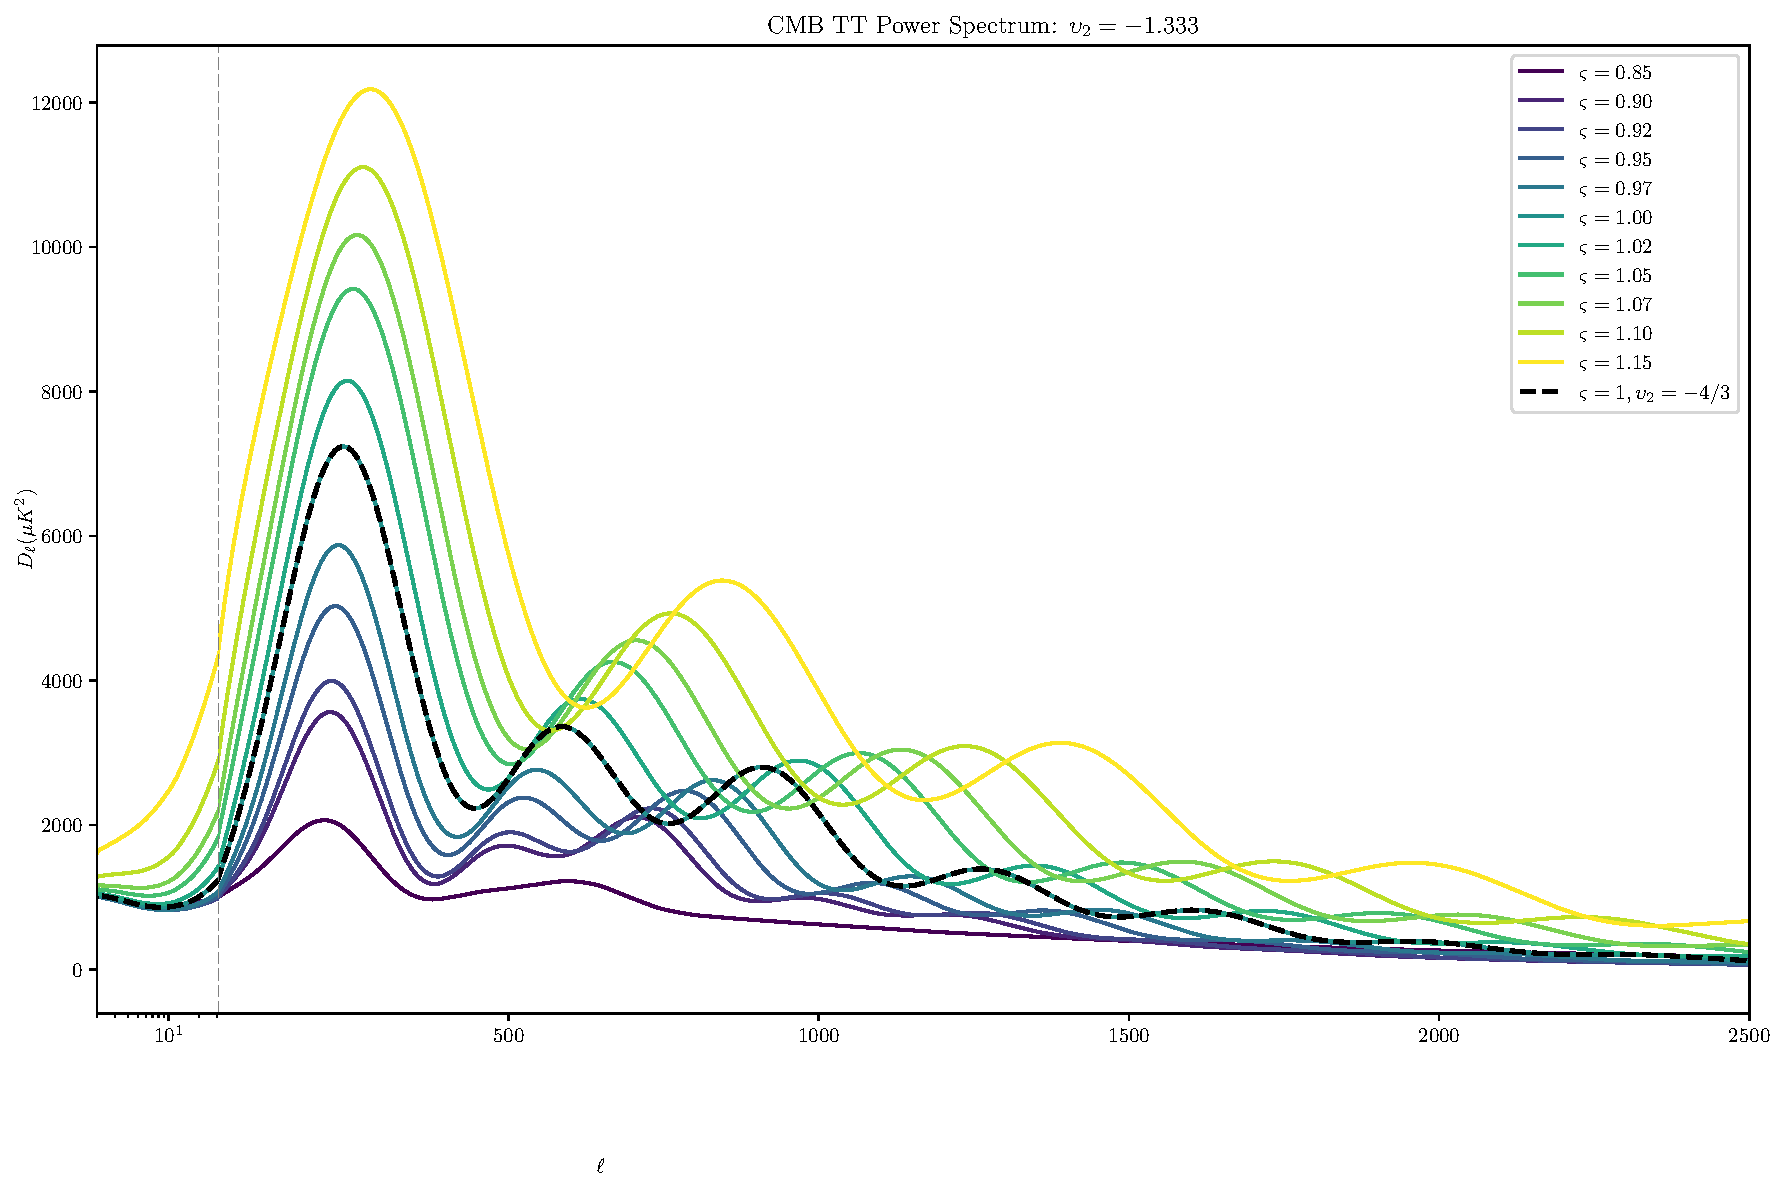
\includegraphics[width=0.95\textwidth]{../Plots/cmb_power_spectrum_varsigma_comparison.pdf}
\caption{CMB TT power spectrum comparison for different values of the stigma parameter $\varsigma$ with fixed $\upsilon_2 = -4/3$. The plot features a dual-scale layout with log scale for low multipoles ($\ell = 2-30$) and linear scale for high multipoles ($\ell = 30-2500$). The reference case $\varsigma = 1.0, \upsilon_2 = -4/3$ is highlighted with a black dashed line. The expanded parameter range includes values: $[0.85, 0.9, 0.92, 0.95, 0.97, 1.0, 1.02, 1.05, 1.07, 1.1, 1.15]$.}
\label{fig:cmb_varsigma}
\end{figure}

\subsubsection{$\upsilon_2$ Parameter Variation}

\begin{figure}[H]
\centering
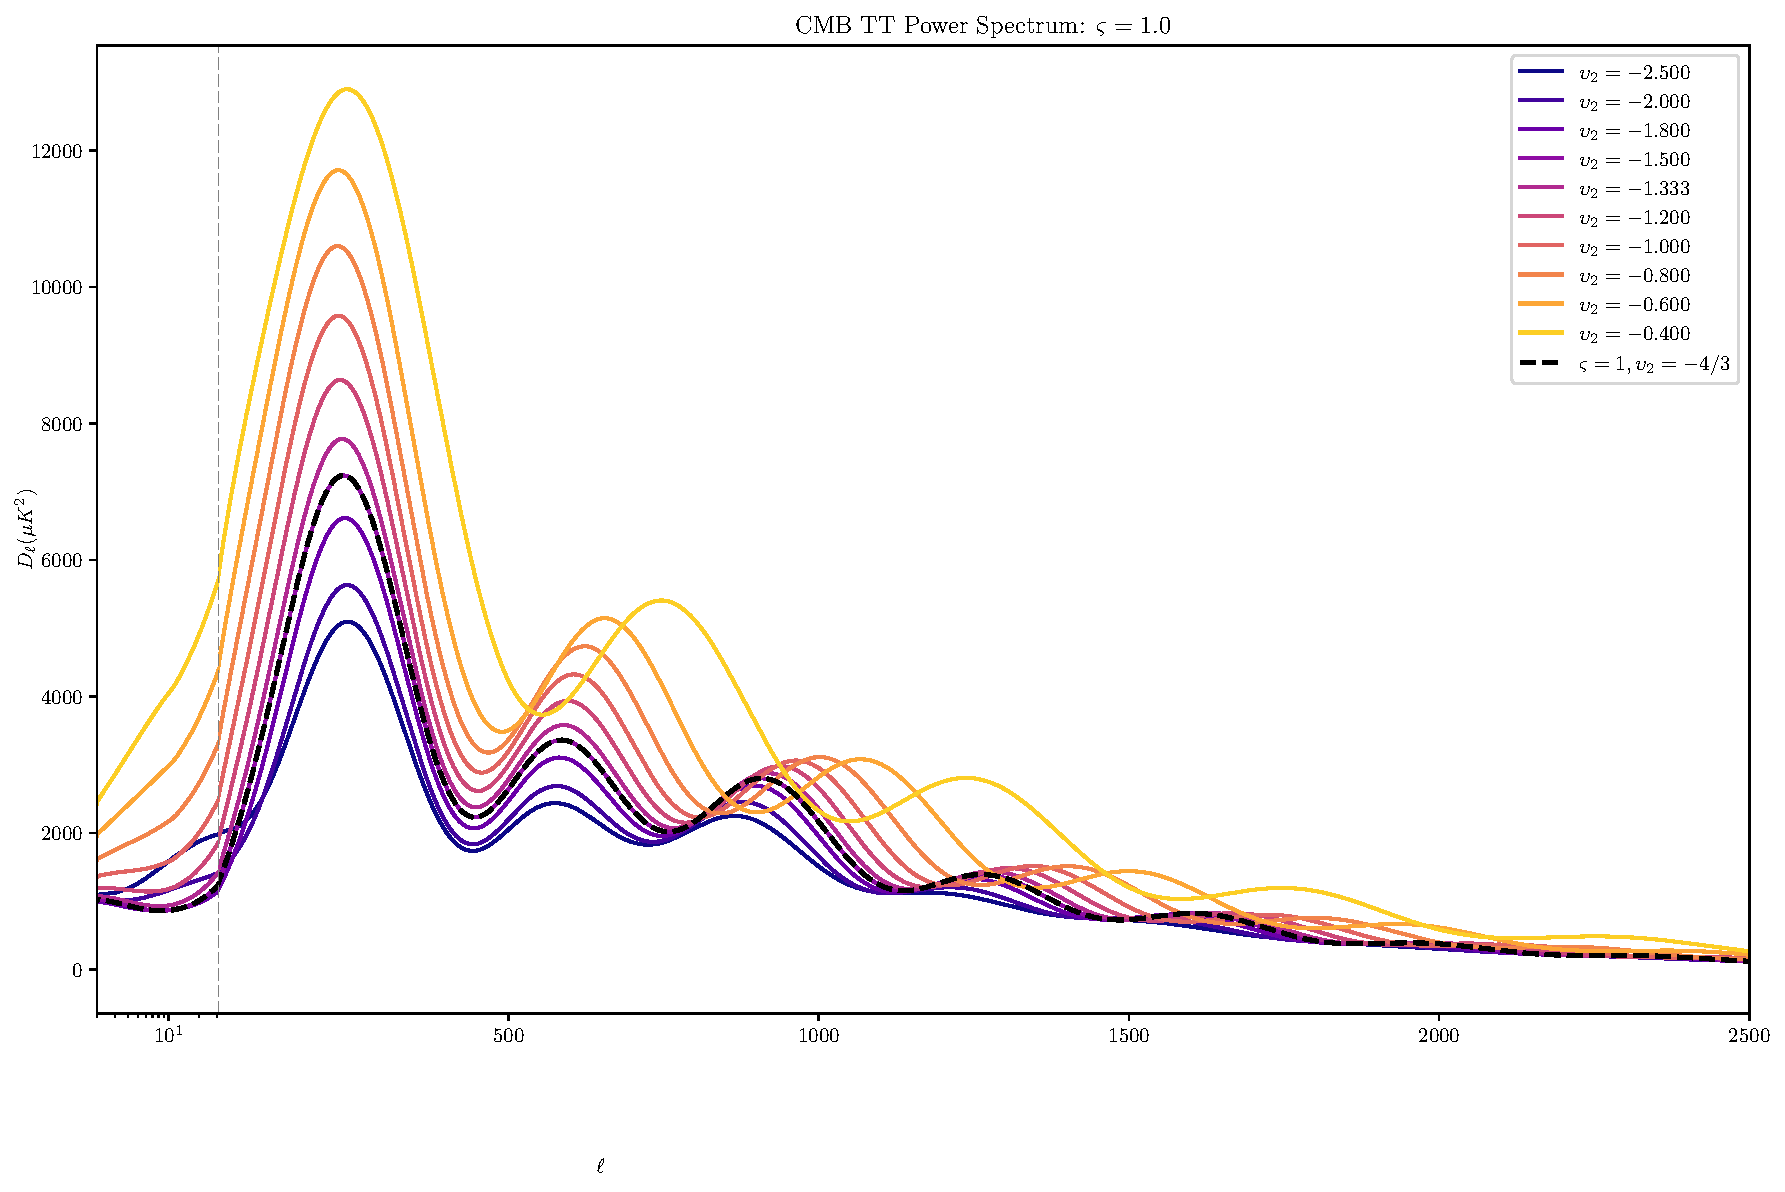
\includegraphics[width=0.95\textwidth]{../Plots/cmb_power_spectrum_upsilon2_comparison.pdf}
\caption{CMB TT power spectrum comparison for different values of the coupling parameter $\upsilon_2$ with fixed $\varsigma = 1.0$. The dual-scale layout allows detailed examination of both acoustic peaks and damping tail behavior. The reference case is again highlighted in black dashed lines. The parameter range covers: $[-2.5, -2.0, -1.8, -1.5, -4/3, -1.2, -1.0, -0.8, -0.6, -0.4, -0.2]$.}
\label{fig:cmb_upsilon2}
\end{figure}

\subsubsection{Hubble Horizon Analysis}

\begin{figure}[H]
\centering
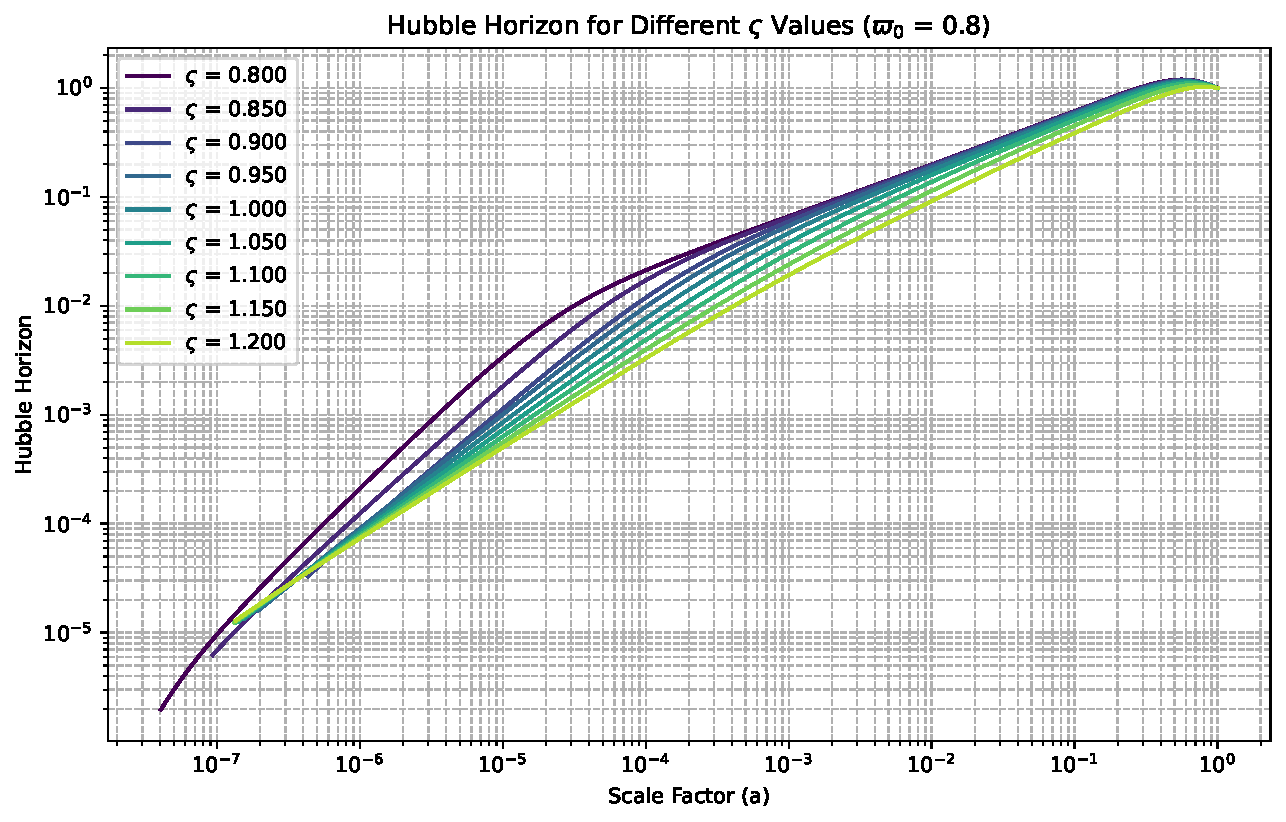
\includegraphics[width=0.95\textwidth]{../Plots/hubble_horizon_varsigma.pdf}
\caption{Hubble horizon evolution for different values of the stigma parameter $\varsigma$ with fixed $\upsilon_2 = -4/3$ and $\varpi_0 = 0.8$. The Hubble horizon is defined as $a/(H \cdot a_0 / (h \cdot 100))$ and shown as a function of scale factor $a$. Both axes use logarithmic scaling to capture the full range of cosmological evolution. Only parameter values satisfying the validity constraints $\varsigma > \varpi_0^2$ and $\varsigma(5 + 4\varsigma(-2 + \varpi_0^2)) < \varpi_0^2$ are included.}
\label{fig:hubble_horizon_varsigma}
\end{figure}

\begin{figure}[H]
\centering
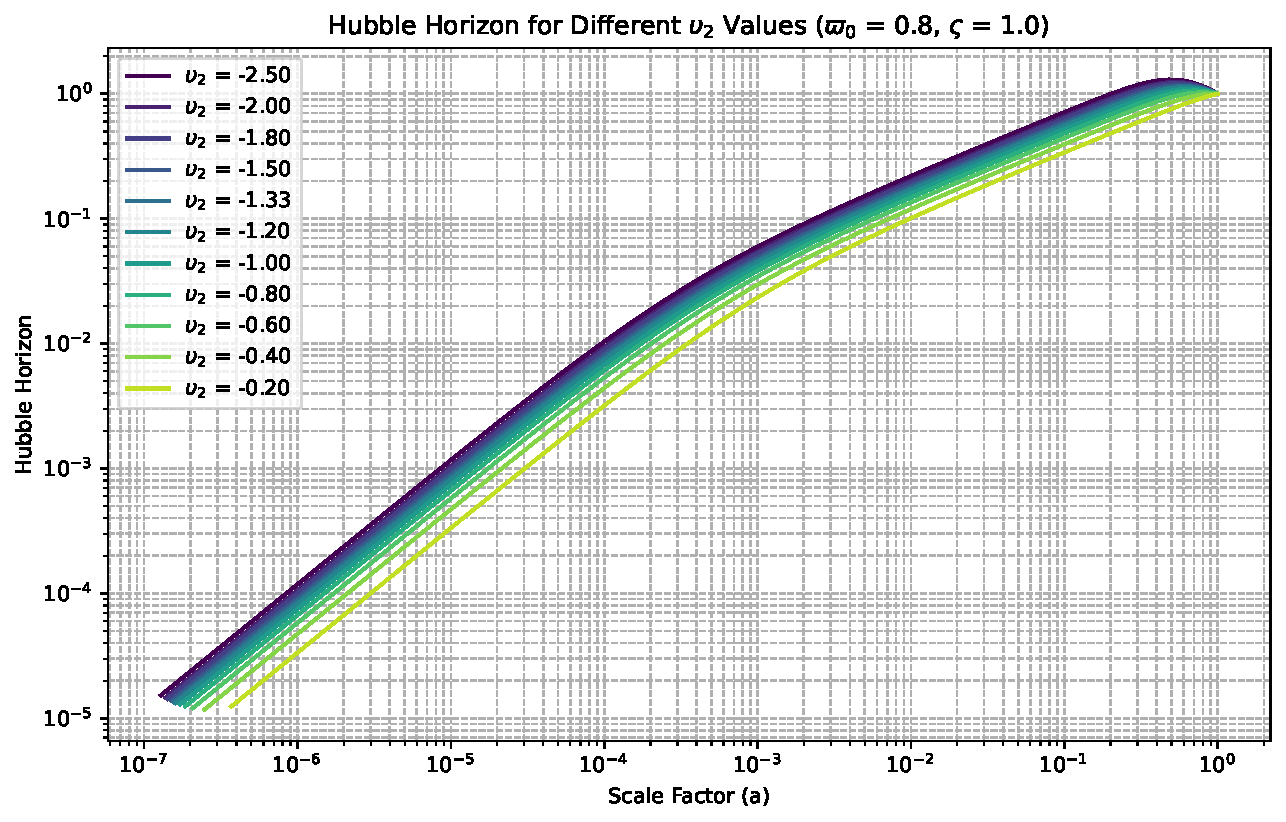
\includegraphics[width=0.95\textwidth]{../Plots/hubble_horizon_upsilon2.pdf}
\caption{Hubble horizon evolution for different values of the coupling parameter $\upsilon_2$ with fixed $\varsigma = 1.0$ and $\varpi_0 = 0.8$. The plot demonstrates how the coupling strength affects the cosmological expansion history and horizon structure. Parameter values range from $-2.5$ to $-0.2$, showing the sensitivity of horizon evolution to the theory's coupling parameter.}
\label{fig:hubble_horizon_upsilon2}
\end{figure}

\subsubsection{Dark Energy Equation of State}

\begin{figure}[H]
\centering
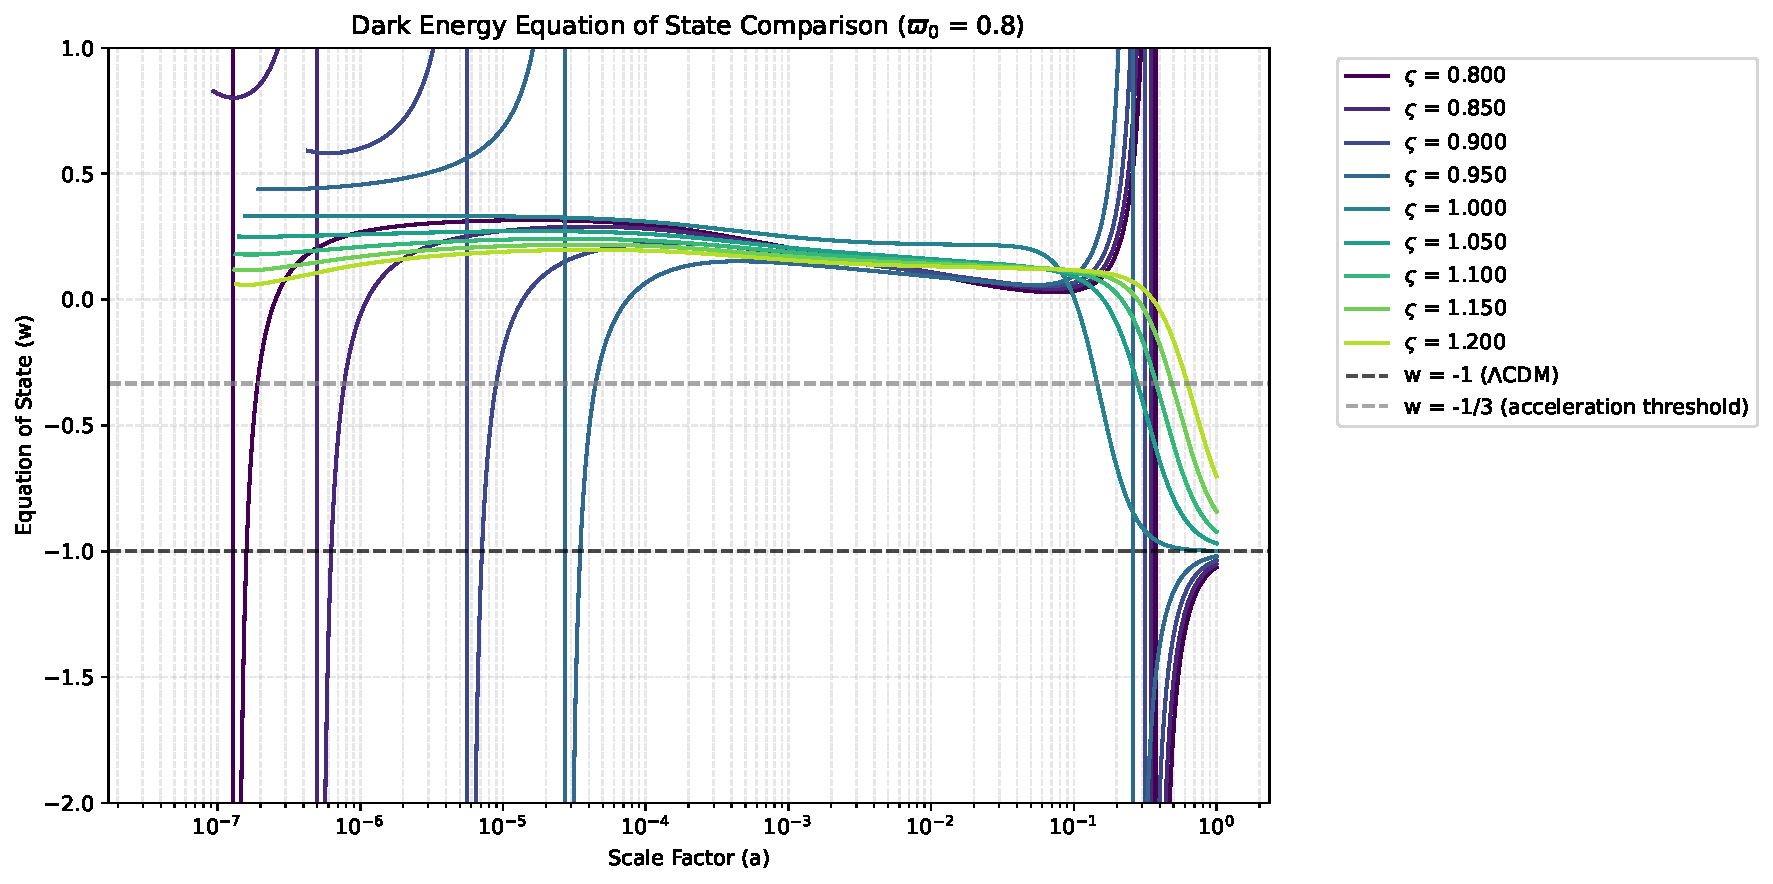
\includegraphics[width=0.95\textwidth]{../Plots/w_comparison_varsigma.pdf}
\caption{Dark energy equation of state parameter $w = P_{DE}/\rho_{DE}$ as a function of scale factor for different $\varsigma$ values with fixed $\upsilon_2 = -4/3$. The horizontal dashed lines indicate $w = -1$ ($\Lambda$CDM behavior) and $w = -1/3$ (acceleration threshold). The Stigma theory predicts time-varying dark energy with distinct evolution patterns depending on the stigma parameter value. The scale factor is shown on a logarithmic scale to capture both early and late-time behavior.}
\label{fig:w_comparison_varsigma}
\end{figure}

\begin{figure}[H]
\centering
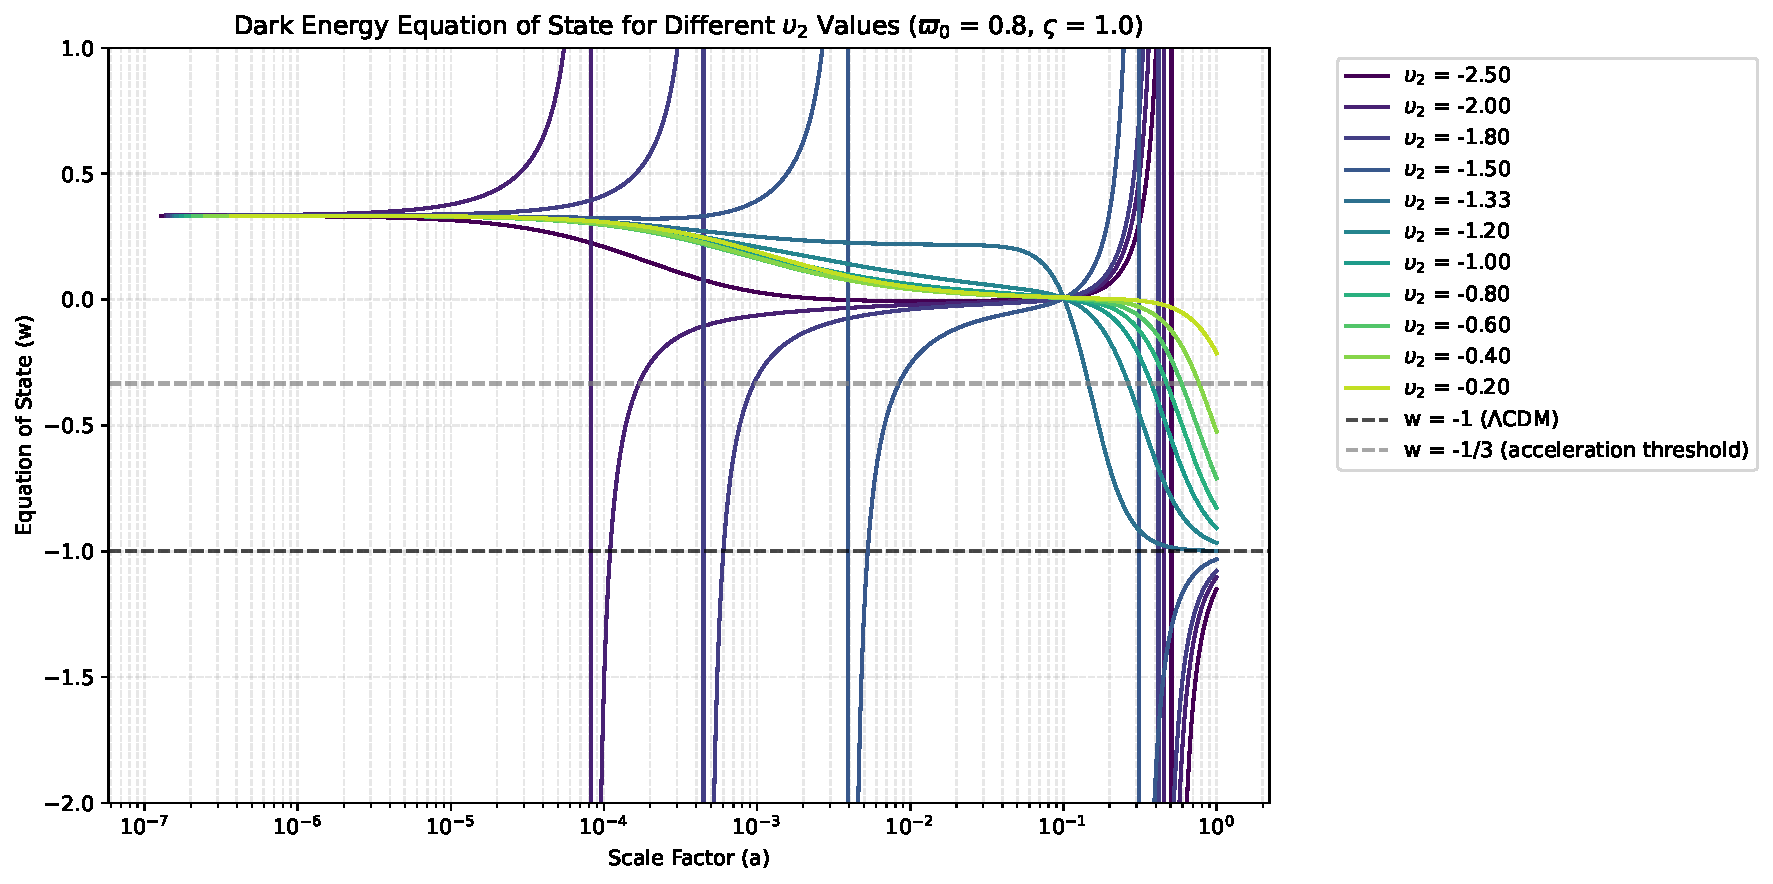
\includegraphics[width=0.95\textwidth]{../Plots/w_comparison_upsilon2.pdf}
\caption{Dark energy equation of state parameter $w$ evolution for different $\upsilon_2$ values with fixed $\varsigma = 1.0$. The plot reveals how the coupling parameter influences the dark energy dynamics, with some parameter choices leading to phantom dark energy ($w < -1$) or even positive $w$ values during certain epochs. The reference lines help identify when the universe transitions between decelerated and accelerated expansion phases.}
\label{fig:w_comparison_upsilon2}
\end{figure}

\subsection{Key Observational Features}

The comprehensive analysis reveals several distinctive features of the Stigma Q-torsion theory across multiple observables:

\subsubsection{CMB Power Spectrum Features}
\begin{itemize}
\item \textbf{Acoustic Peak Modifications}: The positions and amplitudes of acoustic peaks are sensitive to both $\varsigma$ and $\upsilon_2$, providing potential observational signatures
\item \textbf{Damping Tail Behavior}: High-$\ell$ behavior differs from $\Lambda$CDM, particularly for extreme parameter values
\item \textbf{Low-$\ell$ Suppression/Enhancement}: The large-scale power can be either suppressed or enhanced depending on parameter choices
\item \textbf{ISW Effect Modifications}: The modified expansion history affects the integrated Sachs-Wolfe effect at low multipoles
\end{itemize}

\subsubsection{Hubble Horizon and Expansion History}
\begin{itemize}
\item \textbf{Modified Horizon Evolution}: The Hubble horizon shows distinct scaling behavior compared to standard cosmology
\item \textbf{Parameter Sensitivity}: Both $\varsigma$ and $\upsilon_2$ significantly affect the expansion rate and horizon structure
\item \textbf{Validity Constraints}: The theory imposes specific constraints on parameter combinations for physical solutions
\item \textbf{Scale Factor Dependence}: The horizon evolution exhibits complex behavior across different cosmological epochs
\end{itemize}

\subsubsection{Dark Energy Dynamics}
\begin{itemize}
\item \textbf{Time-Varying Equation of State}: Unlike $\Lambda$CDM's constant $w = -1$, Stigma theory predicts evolving dark energy
\item \textbf{Phantom Dark Energy}: Some parameter combinations yield $w < -1$, indicating phantom dark energy behavior
\item \textbf{Acceleration Transitions}: The theory allows for transitions between decelerated and accelerated expansion phases
\item \textbf{Early-Time Dynamics}: The equation of state shows distinctive early-universe behavior that differs from late-time evolution
\item \textbf{Parameter-Dependent Trajectories}: Different $\{\varsigma, \upsilon_2\}$ combinations produce qualitatively different $w(a)$ evolution
\end{itemize}

\subsection{Theoretical Implications}

The power spectrum analysis demonstrates that:

\begin{enumerate}
\item The Stigma Q-torsion theory produces observationally distinct CMB signatures
\item Parameter values near the reference case ($\varsigma \sim 1, \upsilon_2 \sim -4/3$) yield spectra compatible with observations
\item Extreme parameter values lead to significant deviations that could be ruled out by current CMB data
\item The theory provides a framework for testing modified gravity through precision cosmology
\end{enumerate}

\subsection{Future Observational Tests}

These results suggest several avenues for observational constraints:

\begin{itemize}
\item \textbf{Planck Data Analysis}: Compare our theoretical spectra with Planck temperature and polarization data
\item \textbf{Parameter Estimation}: Use MCMC methods to constrain $\{\varsigma, \upsilon_2\}$ from observational data
\item \textbf{Model Selection}: Apply Bayesian model comparison to test Stigma theory against $\Lambda$CDM
\item \textbf{Cross-correlations}: Study temperature-polarization and polarization-polarization spectra for additional constraints
\end{itemize}

\end{document}
